
\documentclass[conference]{IEEEtran}
\usepackage{cite}
\usepackage{graphicx}
\usepackage{amsmath}
\usepackage{enumerate}
\usepackage{xcolor}
\usepackage{pgfplots}
\usepackage{tikz}

\definecolor{bblue}{HTML}{4F81BD}
\definecolor{rred}{HTML}{C0504D}
\definecolor{ggreen}{HTML}{9BBB59}
\definecolor{ppurple}{HTML}{9F4C7C}

% correct bad hyphenation here
\hyphenation{op-tical net-works semi-conduc-tor}


\begin{document}

\title{BUMPER: A Bug-Fix Search Engine}


\author{\IEEEauthorblockN{Mathieu Nayrolles, }
\IEEEauthorblockA{Software Behaviour Analysis (SBA) Research Lab\\
ECE, Concordia University\\
Montreal, Canada\\
m\_nayrol@ece.concordia.ca}
\and
\IEEEauthorblockN{Abdelwahab Hamou-Lhadj}
\IEEEauthorblockA{Software Behaviour Analysis (SBA) Research Lab\\
ECE, Concordia University\\
Montreal, Canada\\
abdelw@ece.concordia.ca}}

% make the title area
\maketitle

% As a general rule, do not put math, special symbols or citations
% in the abstract
\begin{abstract}
  In the last decade, the use of bug tracking tools
  have been adopted by both open-source and industry to take
  advantage of their various features.
 Bug tracking systems such
  as Bugzilla or Jira have grown to contain hundreds of thousands
  of bugs and provide crucial data to several active research fields
  such as bug reproduction, bug triaging, identification of
  duplicate bug, bug comprehension, and empirical studies.
 Easy
  access to the combined histories of all major open-source
  projects will save developers’ time and efforts when facing a bug
  or crash.
 The fixes to these bugs, however, are contained in
  software versioning and revision systems and not in the bug
  tracking system.
 Furthermore, each software project comes with
  its own bug report and source versioning system.
 As a result,
  developers tend to reinvent the wheel instead of leveraging
  known solutions to similar problems.
 In this paper, we present
  an online tool called BUMPER (BUg Metarepository for
  dEvelopers and Researchers) that aims to ease this process and
  allows natural language searches in bug reports, commit
  messages and source code all together at https://bumper-app.com/.
  Currently, BUMPER contains more than 380 projects,
  100,000 resolved/fixed bugs and almost 70,000 changesets from
  Netbeans and the Apache Software foundation’s softwares.
  BUMPER is designed to be easily extensible to contain bugs and
  fixes from other bug and version control systems.

\end{abstract}


\IEEEpeerreviewmaketitle


\section{Introduction}

Debugging programs, during their creations or at maintenance time is challenging \cite{Pressman2005} and taxing -- Studies have shown that the cost of software maintenance can reach up to 70\% of the overall cost of the software development process.

 When facing a yet unknown bug, one might want to leverage decades of open-source software history in order to find a solution. Indeed, chances are a similar bug or crash has already been fixed somewhere in an open-source project.

 However, each open-source project host its data on a different data repository and using different bug tracking and source code management systems. Moreover,   these systems have different interfaces to access data.
 The data is not represented in a uniform way either.
 This is further complicated by the fact that bug tracking tools and code versioning systems are not necessarily connected.
 The former follows the life of the bug itself and not its fixes, which are managed by the latter.
 As a general practice, developers create a link between the bug report system and the source versioning tool by either writing the bug #ID in their commit message or add a link towards the changeset as a comment in the bug report system.

 As a result, one would have to search the source code versioning system repository to find candidate solutions.
 Moreover, developers mainly use classical search engines that index specialized sites such as StackOverflow.

 However, specialized sites are organized in the form of question-response where one explain his problem and gets answers from the community.
 While the answers are often accurate and precise, they do not leverage the history of open-source software that has been shown to provide useful insight to help with many maintenance activities such as bug fixing \cite{Weiß2007} \cite{Saha2014} , bug reproduction \cite{Chen2013a} \cite{Artzi2008} \cite{Jin2012}, fault analysis \cite{Nessa2008}, etc.
 For the present time, analyzing the bugs and their fixes from different sources require going back and forth between diverse tools, creating parsers, mapping data from a repository to another, etc.
 These tasks are not only time consuming but add no value to the analysis itself.

 In this paper, we introduce BUMPER (BUg Metarepository for dEvelopers and Researchers), a web-based infrastructure that can be used by software developers and researchers to access data from diverse repositories using natural language query in a transparent manner, regardless of where the data was originally created and hosted.

 The idea behind BUMPER is that it can connect to any bug tracking and source code versioning system and download the data into a single database.
 BUMPER uses a web-based interface that allows users to search the aggregated database by expressing queries through a single access point.
 This way, users can focus on the analysis itself and not on the way data is represented or where it is located.

 To create an approach that will efficiently help the community at debugging time we first ask computer science students, professionals and practitioners to answer a short survey about how they face unknown bug, crash or exception.

 Even thought their answers, presented in Section \ref{sec:Tools and methods used to fix unknown bug} were not surprising, we still used them to build an approach that fits the needs of the community and built a dataset of 840 open source projects belonging to five major open-source institutions with more than 100,000 resolved/fixed and with 60,000 changesets that were involved in fixing them from Eclipse, Netbeans, Gnome, Github and the Apache Software foundation's software.

 BUMPER supports many features including: (1) the ability to search large data repositories very efficiently using both natural languages and a specialized query language, (2) the mapping between the bug reports and the code involved to fix it, (3) the ability to export the search results in Json, CSV and XML formats.

 Finally, we went back to the community and ask them to solve bugs and crashes using their habitual habits and using BUMPER. The results indicate that our approach reduces the amount of data-sources to be visited in order to find a suitable solution for the bug at hand and therefore, speeding up the debugging and maintenances processes.

 The remaining of this paper is organized as follows. First we present the results of our first survey aiming to understand the behavior of developers when facing a bug in Section \ref{sec:Tools and methods used to fix unknown bug}. Then, we present background informations about bug tracking and code versions systems in Section \ref{sec:background}. BUMPER itself is presented in terms of its architecture, metadata and API in section \ref{sec:Bumper Components}. Our second survey, presenting the advantages of BUMPER compared to habitual ways of doing maintenance and bug fixing is the subject of Section \ref{sec:Experiments}. Finally, we present related works and concluding remarks in Sections \ref{sec:Related Works} and \ref{sec:conclusion}, respectively.

\section{Tools and methods used to fix unknown bug}
\label{sec:Tools and methods used to fix unknown bug}

In this section we present the results of a two-rounds survey we conduct with students and developers in order to understand what are their habits when dealing with an yet unknown bug, exception or crash. In the first round, we ask participant to answer the following two question: (1) \textit{When facing an unknown bug, crash or exception, where do you look for informations ?} and (2) \textit{When facing an unknown bug, crash or exception, what are you searching for ?}. We then summarized their answers and took the most popular ones to build the following multi-choices survey:

\begin{enumerate}
  \item When facing an unknown bug, crash or exception, where do you look for informations ?
  \begin{enumerate}[a)]
    \item Online search engines (Google, Bing, ...).
    \item Online specialized websites (Stackoverflow, ...)
    \item Offline search (Books, Slides, ...).
    \item Official documentation of the project / programming languages / api (Offline and Online).
    \item Other.
  \end{enumerate}
  \item When facing an unknown bug, crash or exception, what are you searching for ?
  \begin{enumerate}[a)]
    \item How to do X.
    \item The exception yield by the crash / bug.
    \item Official documentation of the project / programming languages / api (Offline and Online).
  \end{enumerate}
\end{enumerate}

We submitted this survey to a total of 150 peoples and got 89 responses (59\%). Respondent to our surveys have been classified into four distinct groups: undergraduate (42) and graduate (25) students in computer sciences, electrical and computer engineering and software engineering. The two last groups are junior developers (15) (0-3 years of experience) and intermediate or senior developers (7) (3+ years of experience).
We report the results of our surveys using descriptive statistics (percentage) and present the results for each of our four surveyed groups.

Figure~\ref{fig:infos} presents the results of our first question : \textit{When facing an unknown bug, crash or exception, where do you look for informations ?}
73\%, 65\%, 75\% and 58\% of Undergraduate, Graduate, Junior developers and intermediate or senior developers, respectively, indicate that they use \textit{Online search engines} such as Google or Bing to resolve yet unknown bug.
In the meantime, 5\%, 25\%, 12\% and 28\% of Undergraduate, Graduate, Junior developers and intermediate or senior developers, respectively, indicate that they use \textit{Online specialized websites} such as StackOverflow.
Interestingly, some of the respondent that were surveyed offline and answered that they use \textit{Online search engines} search engines told us that the best answer was often hosted on a \textit{Online specialized websites} such as StackOverflow. \textit{Offline} (Books, slides, ...) and \textit{documentation} searches reach 22\% and 0\%, 5\% and 2\%, 5\% and 8\% and 8\% and 12\% for  Undergraduate, Graduate, Junior developers and intermediate or senior developers, respectively.

\begin{figure}[h!]
  \centering

  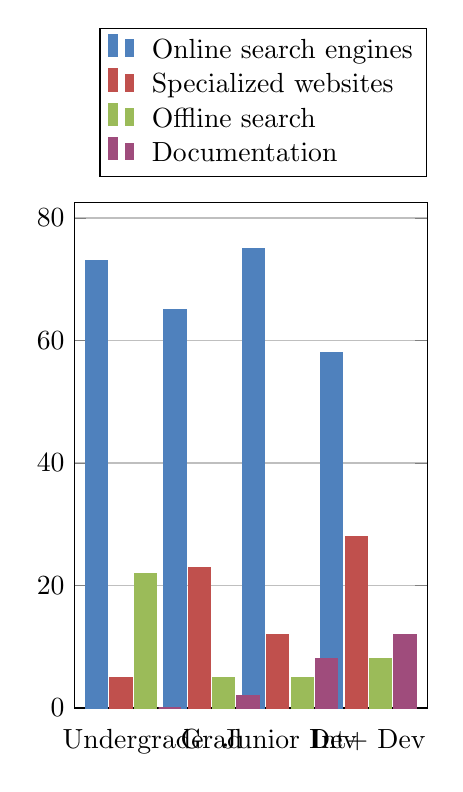
\begin{tikzpicture}
   \begin{axis}[
       width  = 0.5*\textwidth,
       height = 8cm,
       major x tick style = transparent,
       ybar=2*\pgflinewidth,
       bar width=8pt,
       ymajorgrids = true,
       symbolic x coords={Undergrade, Grad, Junior Dev, Int+ Dev},
       xtick = data,
       scaled y ticks = false,
       enlarge x limits=0.25,
       ymin=0,
       legend cell align=left,
       legend style={
               at={(1,1.05)},
               anchor=south east,
               column sep=1ex
       }
   ]
       \addplot[style={bblue,fill=bblue,mark=none}]
           coordinates {(Undergrade, 73) (Grad,65) (Junior Dev,75) (Int+ Dev,58)};

       \addplot[style={rred,fill=rred,mark=none}]
             coordinates {(Undergrade, 5) (Grad,23) (Junior Dev,12) (Int+ Dev,28)};

       \addplot[style={ggreen,fill=ggreen,mark=none}]
             coordinates {(Undergrade, 22) (Grad,5) (Junior Dev,5) (Int+ Dev,8)};

       \addplot[style={ppurple,fill=ppurple,mark=none}]
           coordinates {(Undergrade, 0) (Grad,2) (Junior Dev,8) (Int+ Dev,12)};

       \legend{Online search engines, Specialized websites, Offline search , Documentation}
   \end{axis}
\end{tikzpicture}

    \caption{Answers to \textit{When facing an unknown bug, crash or exception, where do you look for informations ?} in percentage\label{fig:infos}}
\end{figure}


To summarize, 84.7\% of respondents declared that their first reflex when facing an yet unknown bug was to search for a suitable solution online. These 84.7\% participant were asked to continue the survey with the second question.
To keep our results as qualitative as possible we excluded participants that indicated searching for resources offline as our approach aimed to improve onlime behaviors.

Figure~\ref{fig:keywords} presents the results of our first question : \textit{When facing an unknown bug, crash or exception, what are you searching for ?} 47\%, 32\%, 55\% and 22\% of Undergraduate, Graduate, junior developers and intermediate or senior developers, respectively, indicate that they use a \textit{How to do X} search query when searching solution to resolve yet unknown bug. Another 53\%, 60\%, 37 \% and 67\% of Undergraduate, Graduate, junior developers and intermediate or senior developers, respectively, copy past directly the exception or crash output at hand. Finally, 0\%, 8\%, 8\% and 11\% of Undergraduate, Graduate, junior developers and intermediate or senior developers, respectively search for solution in the online official documentation of the project they are working on.

\begin{figure}[h!]
  \centering

  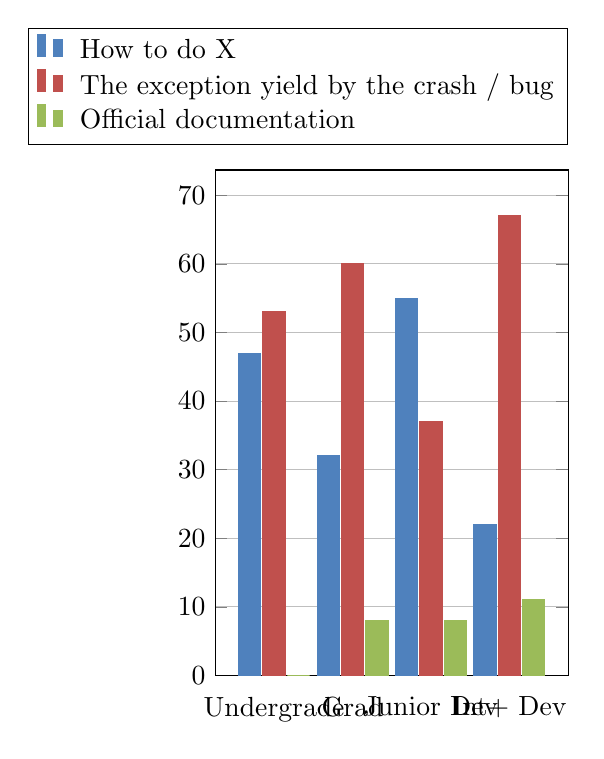
\begin{tikzpicture}
   \begin{axis}[
       width  = 0.5*\textwidth,
       height = 8cm,
       major x tick style = transparent,
       ybar=2*\pgflinewidth,
       bar width=8pt,
       ymajorgrids = true,
       symbolic x coords={Undergrade, Grad, Junior Dev, Int+ Dev},
       xtick = data,
       scaled y ticks = false,
       enlarge x limits=0.25,
       ymin=0,
       legend cell align=left,
       legend style={
               at={(1,1.05)},
               anchor=south east,
               column sep=1ex
       }
   ]
       \addplot[style={bblue,fill=bblue,mark=none}]
           coordinates {(Undergrade, 47) (Grad,32) (Junior Dev,55) (Int+ Dev,22)};

       \addplot[style={rred,fill=rred,mark=none}]
             coordinates {(Undergrade, 53) (Grad,60) (Junior Dev,37) (Int+ Dev,67)};

       \addplot[style={ggreen,fill=ggreen,mark=none}]
             coordinates {(Undergrade, 0) (Grad,8) (Junior Dev,8) (Int+ Dev,11)};


       \legend{How to do X, The exception yield by the crash / bug, Official documentation}
   \end{axis}
\end{tikzpicture}

    \caption{Answers to \textit{When facing an unknown bug, crash or exception, what are you searching for ?} in percentage\label{fig:keywords}}
\end{figure}


To summarize, 93.25 \% of surveyed participant who search solution to an unknown bug or crash online use query composed of \textit{How to do X} or directly copy past their error / exception. Both these information can be found in bug report and bug fixes as described in the next section.


\section{background}
\label{sec:background}

\subsection{Bug Tracking System}
\label{sub:bug-tracking-system}

Open source bug tracking systems allow end-users to directly create BRs to report on system crashes.
These systems are also used by development teams to manage the BRs, and keep track of the fixes.
The lifecycle of a bug in both systems is as follows: After a bug is submitted by an end-user, it is set to the UNCONFIRMED state until it receives enough votes or that a user with the proper permissions modifies its status to “EW.
The bug is then assigned to a developer to fix it.
When the bug is in the ASSIGNED state, developers start working on fixing the bug.
A fixed bug moves to the RESOLVED state.
Developers have five different possibilities to resolve a bug: FIXED, DUPLICATE, WONTFIX, WORKSFORME and INVALID.
Finally, the bug is closed after it is resolved.
A bug can be reopened (set to the REOPENED state) and then assigned again if the initial fix was not adequate (the fix did not resolve the problem).
The elapsed time between the bug is marked as new one and the resolved status is known as the fixing time, we denote the fixing time by BFT.
It usually in days.
If the bug is reopened then the days between the time the bug is reopened and the time it is marked as RESOLVED/FIXED are cumulated.
Bugs can be reopened many times.
The relationship between a BR and the actual fix can be hard to establish and it has been a subject for various research studies (e.g., \cite{Wu2011}\cite{Antoniol2002}).
While it is considered a good practice to link each BR with the source code repository by indicating the bug id on the commit message, more than half of the bugs in our dataset are not linked to a commit.
We exclude these bugs in this study and only consider the ones that have a commit.
This way, we can establish a link between the bug and its fixes.
A commit contains the number of files changed in all the commits linked to the bug, the number of hunks (the number of lines in a changeset the commits linked to a bug), the number of lines modified in all the commits.
We use this data to construct BUMPER metamodel.


\subsection{Version Constrol System}
\label{sub:Version Constrol System}

Version control systems are used to maintain the versions of files such as source code and other software artifacts.
Many software tools have been created to help practitioners manage the versions of their software artifacts.
Each evolution of a software is a version (or revision) and each version (revision) is linked to the one before through modifications of software artifacts.
These modifications consist of updating, adding or deleting software artifacts can be referred as diff, patch or commit.
Each diff, patch or commit own the following characteristics:

\begin{itemize}
  \item  Number of Files: The number of software artifacts that have been modified, added or deleted.
  \item Number of Hunks: The number of consecutive block of modified, added or deleted lines in textual files.
  \item Hunks are useful to determine, in each file, how many different places the developer has modified.
  \item Number of Churns: The number of lines modified.
  However, the churn value for a line change should be at least two as the line had to be deleted first and then added back with the modification
\end{itemize}

\section{Bumper Components}
\label{sec:Bumper Components}

Figure~\ref{fig:bumper-snapshot}   shows BUMPER’s main interface.
BUMPER aggreagates data from various bug tracking and version control systems that can be efficiently accessible using a webbased interface.
Currently, BUMPER supports 380 projects, more than 100,000 resolved/fixed and with 60,000 changesets from Netbeans and the Apache Software foundation’s softwares.
It can readily be extended to support other systems.
Using BUMPER, software engineers can query multiple repositories and save the data in various formats including Json, CSV, and XML for further analysis.

\begin{figure}[h!]
  \centering
    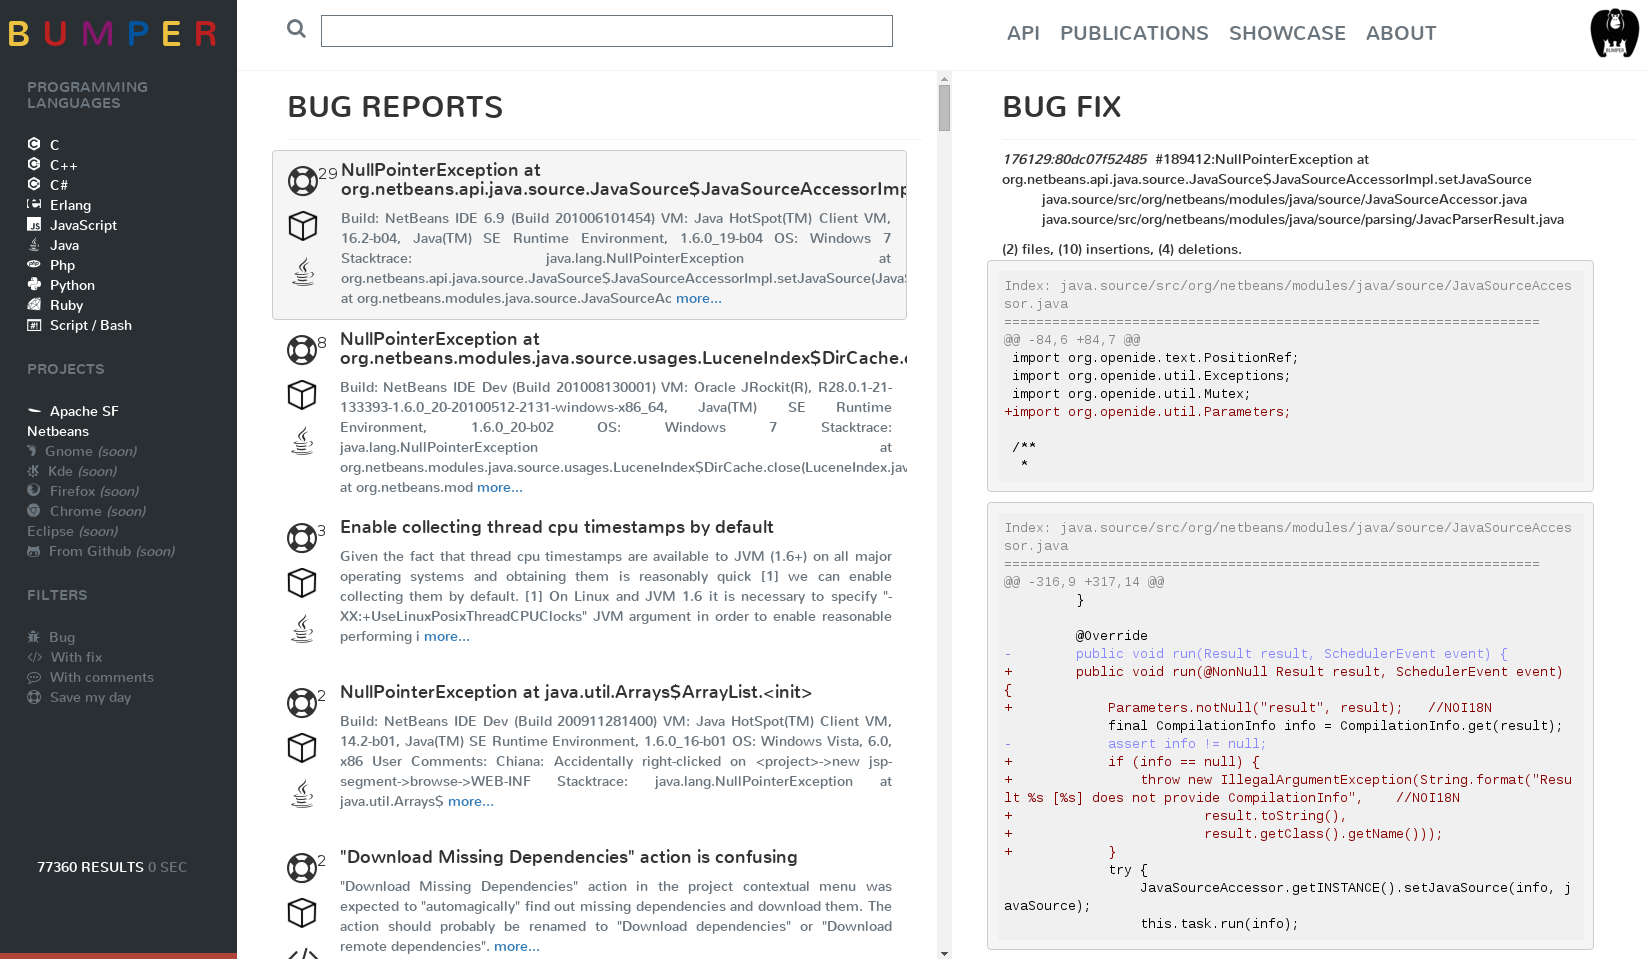
\includegraphics[width=0.5\textwidth]{media/interface.png}
    \caption{ BUMPER Snapshot.\label{fig:bumper-snapshot}}
\end{figure}

\subsection{BUMPER Architecture}
\label{sub:BUMPER Architecture}

Figure~\ref{fig:bumper-architecture} shows the overall architecture of BUMPER.
BUMPER relies on a highly scalable architecture composed
of two Virtual Private Servers (VPS), hosted on a physical
server.
The first server, on the left, handles the web requests and
runs three distinct components: Pound, Varnish, and NginX.
Pound is a lightweight open source reverse proxy program
and application firewall.
It also serves to decode https to request to http.
Translating an https request to http allows us to save the https decryption time required on each step.
Pound also acts as a load-balancing service for the lower levels.
The translated requests are then handled by Varnish.
Varnish is an http accelerator designed for content-heavy and dynamic websites.
It caches requests that come in and serves the Web requests from the cache is the cache is still valid.
NginX (pronounced engine-x) is a web-server that was developed with a particular focus on high concurrency, high performances, and low memory usage.
The second VPS also uses Pound for the same reasons and SolrCloud.
SolrCloud is the scalable version of Apache Solr where the data can be separated into shards (e.g chunk of manageable size).
Each shard can be hosted on a different server but still indexed in a central repository.
Hence, we can guarantee a low query time while exponentially increasing the data.
Finally, Lucene is the full text search engine powering Solr.

\begin{figure}[h!]
  \centering
    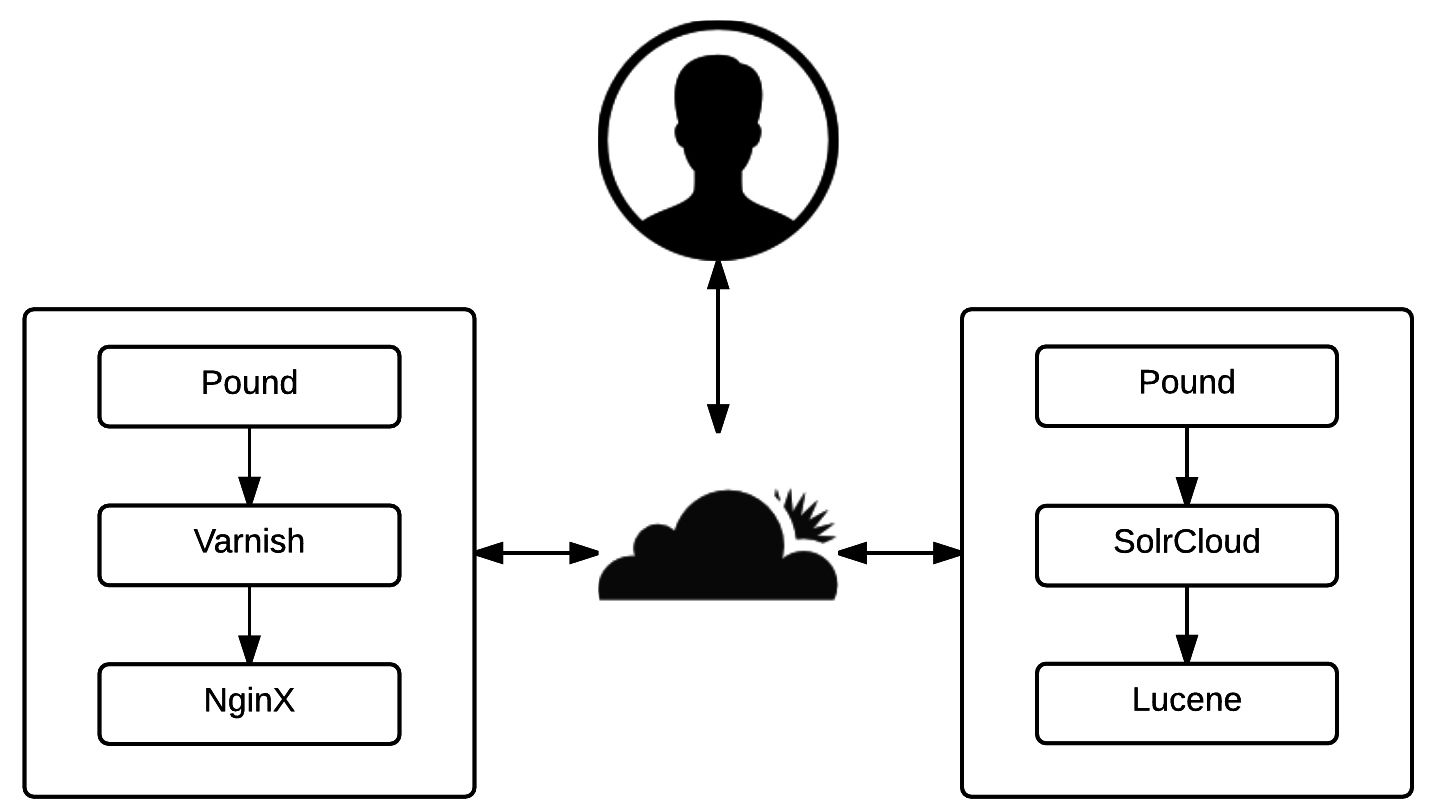
\includegraphics[width=0.4\textwidth]{media/archi.png}
    \caption{BUMPER Architecture.\label{fig:bumper-architecture}}
\end{figure}

\subsection{BUMPER Metadata}
\label{sub:BUMPER Metadata}

Figure~\ref{fig:bumper-metamodel}  shows the core BUMPER metamodel, which captures the common dat elements used by bug tracking and control version systems.
An issue (task) is characterized by a date, title, description, and a fixing time.

\begin{figure*}
  \centering
  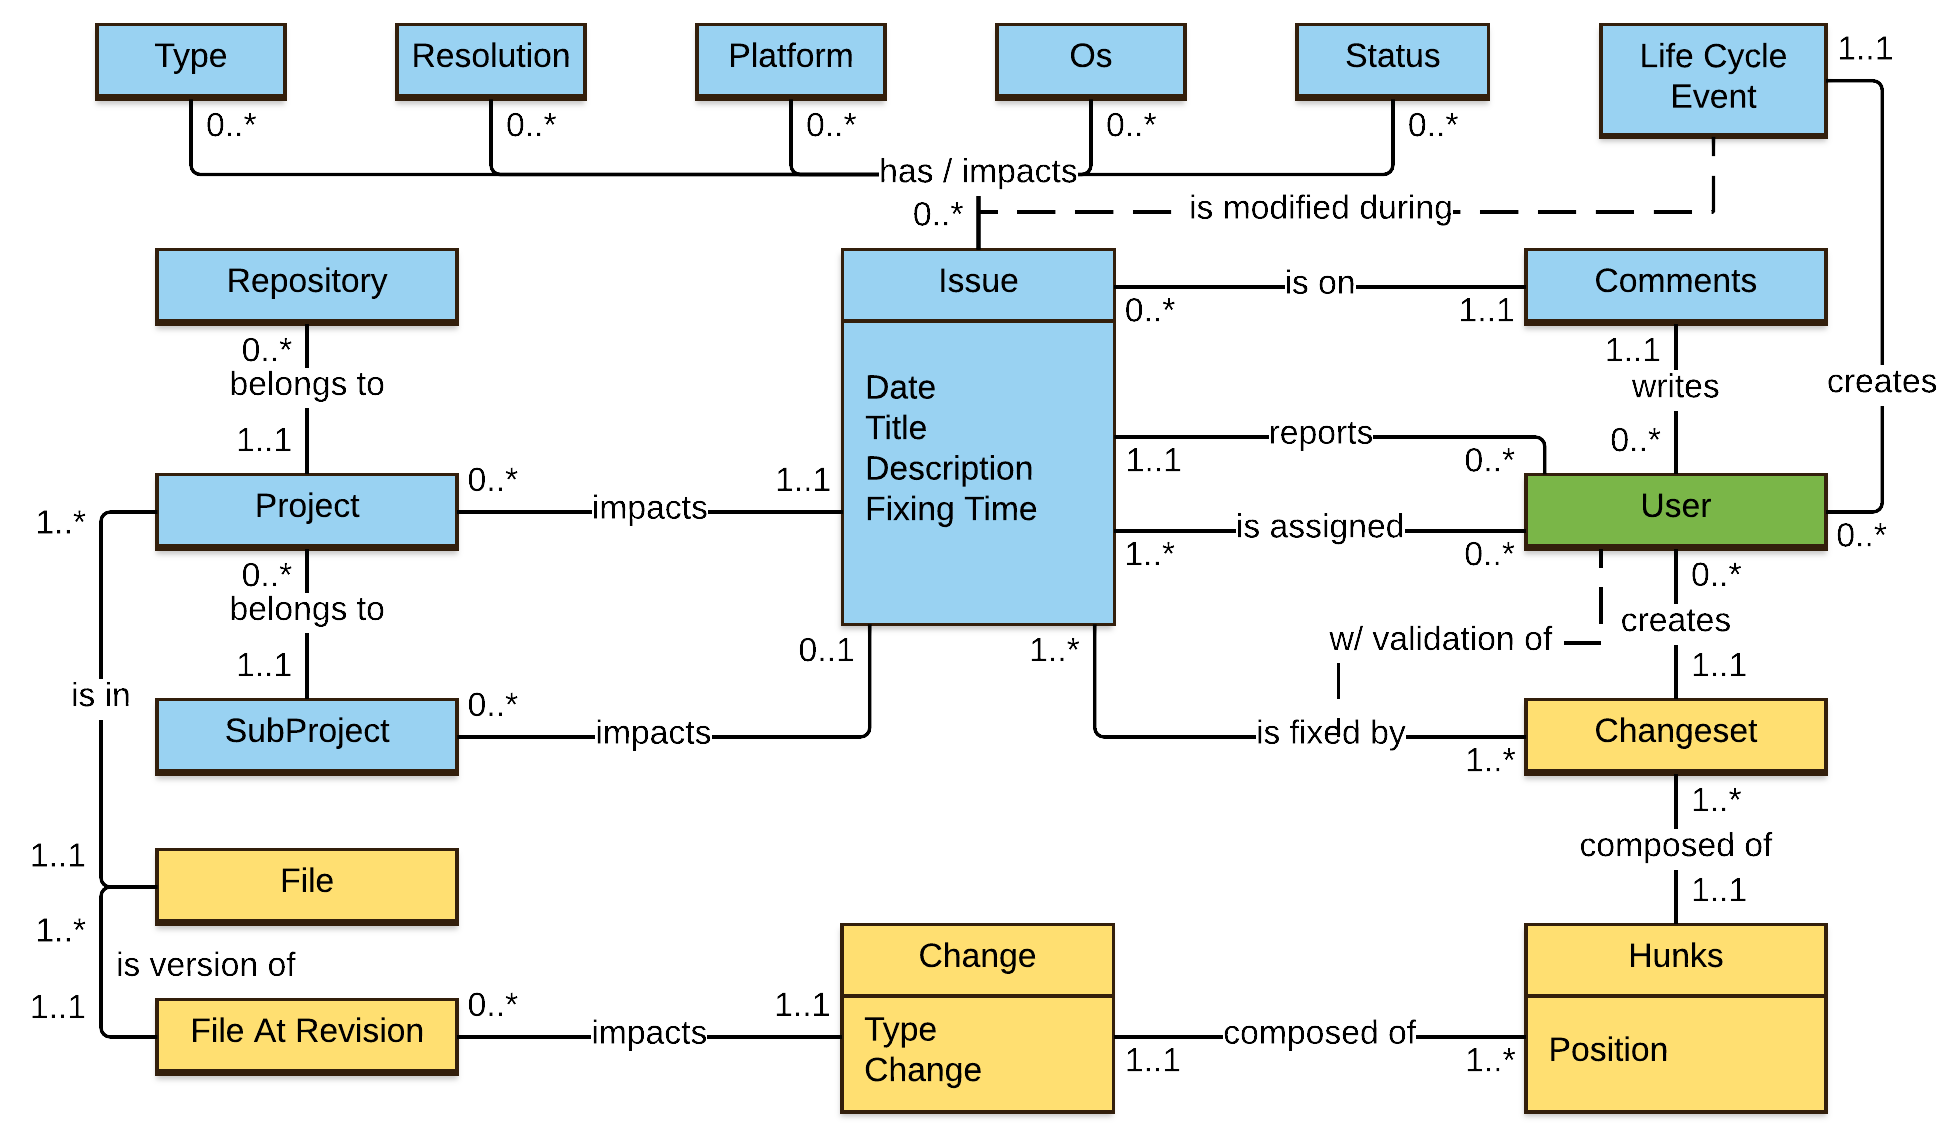
\includegraphics[width=0.8\textwidth]{media/Bumper-Model.png}
  \caption{BUMPER Metamodel\label{fig:bumper-metamodel}}
\end{figure*}

Issues are reported (created) by and assigned to users.
Also, issues belong to a project that is in a repository and might be composed of subprojects.
Users can modify an issue during life cycle events which impact the type, the resolution, the platform, the OS and the status.
Issues are resolved (implemented) by changeset that are composed of hunks.
Hunks contain the actual changes to a file at a given revision, which are versions of the file entity that belongs to a project.
In addition, BUMPER has different indexes over the data in order to provide results in an efficient way.
First of all, each feature of bug reports and bug fixes (number of files, number of hunks, etc.) have their own index.
Furthermore, BUMPER has data indexes over the project name, the sub-project name, the programming language, etc.
Finally, two major indexes are built upon the concatenations of all the textual fields of the bug report and all the textual field (source code included) of a bug fix.
They are named report\_t and fix\_t, respectively.
These indexes are used when querying bug reports or bug fixes using natural language.
Indexes can also be found in relational database management system (RDBMS).
Most modern RDBMS use binary trees to store indexes that keep data sorted and allow searches, insertions, and deletion in a logarithmic time.
Nevertheless, an RDBMS can use only one index per table at the same time.
This said, an RDBMS chooses only one index within the available ones--based on statistics--and uses it to complete the request.
It is highly probable that thousands of records have to be scanned before the RDBMS finds the ones that match the query, especially if there is union or disjunction of records.
Unlike a traditional RDBMS, BUMPER relies on Apache Lucene and uses compressed bitsets to store indexes.
Bitsets are one of the simplest--and older--data structure that contain only 0 and 1.
BUMPER supports binary operations like intersection, AND, OR and XOR that can be performed in a snap on even for thousands and thousands of records.
As an example, if we wish to retrieve bug reports that contain the words null pointer exception and have a changeset containing a try/catch, a binary intersection will be performed between the two sets of documents, which is much faster than selecting bug reports that match null pointer exception first and then checking if they have a changeset containing a a try/catch as in the case of an RDBMS.
This technique comes with a high overhead—comparing to an RDBMS--for indexes update, but, in practice, information retrievals are orders of magnitude faster.
In our case, we want to provide a fast access to decades of open source history.
We periodically update (at night) our indexes when sufficient amount of new data have been downloaded from the bug tracking and source versioning systems BUMPER supports

\subsection{Bumper Query Language and API}
\label{sub:Bumper Query Language and API}

BUMPER supports two query modes: basic and advanced.
The basic query insert users' inputs (YOUR TERMS) in the
following query:

\begin{equation}
\begin{split}
~~(type:"BUG"~AND~report_t:"YOUR~TERMS"~\\
~~AND~-churns:0)
\end{split}
\end{equation}



The first part of the query matches all bug reports
(type:"BUG") that contain YOUR TERMS in the report\_t index
(report\_t:"YOUR TERMS").
Finally, it excludes bug reports that
do not have a fix (-churns:0).
The result of this subquery will be
merged with the following:

\begin{equation}
\begin{split}
~~OR~(\{!parent~which="type:BUG"\}type:~\\
~~"CHANGESET"~AND~fix_t:"YOUR~TERMS"
\end{split}
\end{equation}

This query selects all bugs' changeset--using a parent-child
relationship $(\{!parent which="type:BUG"\}~type:
  "CHANGESET")$ -- and that contain YOUR TERMS in the fix\_t
  index (fix\_t:"YOUR TERMS").
Finally, the results of the two
previous queries will be added to the following subquery:

\begin{equation}
\begin{split}
  OR~(\{!parent~which="type:BUG"\}\ \\
~\{!parent~which="type:CHANGESET"\}\\
~type:"HUNKS"~AND~fix_t:"YOUR TERMS")
\end{split}
\end{equation}

The query selects all the hunks that are child of changsets and
grand-child of bug report $ (\{!parent~which="type:BUG"\}
  \{!parent~which="type:CHANGESET"\}~type:"HUNKS")$
and that
contain YOUR TERMS in the fix\_t index.
The intent of this composed query is search efficiently for
YOUR TERMS in bug reports, commit messages and source
code all together.
The advanced query mode allows users to write their own
query using the indexes they want and the unions or disjunctions
they need.
As an example, using the advanced query mode, one
could write the following:

\begin{equation}
\begin{split}
  (type:"BUG"~AND~report_t:"Exception"~\\
~~AND~(project:"Axis2"~OR~project:"ide")~\\
~~AND~(reporter:"Rich"~OR~resolution:"fixed")~\\
~~AND~(severity:"Major"~OR~fixing_time:[10~TO~*])~\\
~~AND~-churns:0)
\end{split}
\end{equation}

This query finds all bug reports that contain Exception in the
report\_t index (first line) and belong to the Axis2 or the ide
project (line 2) and have been reported by someone named Rich
or have been fixed as a resolution (third line) and that have a
Major severity or a fixing time greater than 10 days (fourth line)
and have a fix (fifth line).
More examples of the API’s usage can
be found at https://bumper-app.com/api.


\subsection{Bumper Data Repository}
\label{sub:Bumper Data Repository}

Figure~\ref{fig:data-collection}  illustrates the process of collecting
data from various repositories and use them in BUMPER.
We show the process using the repositories currently supported by BUMPER.

\begin{figure}[h!]
  \centering
    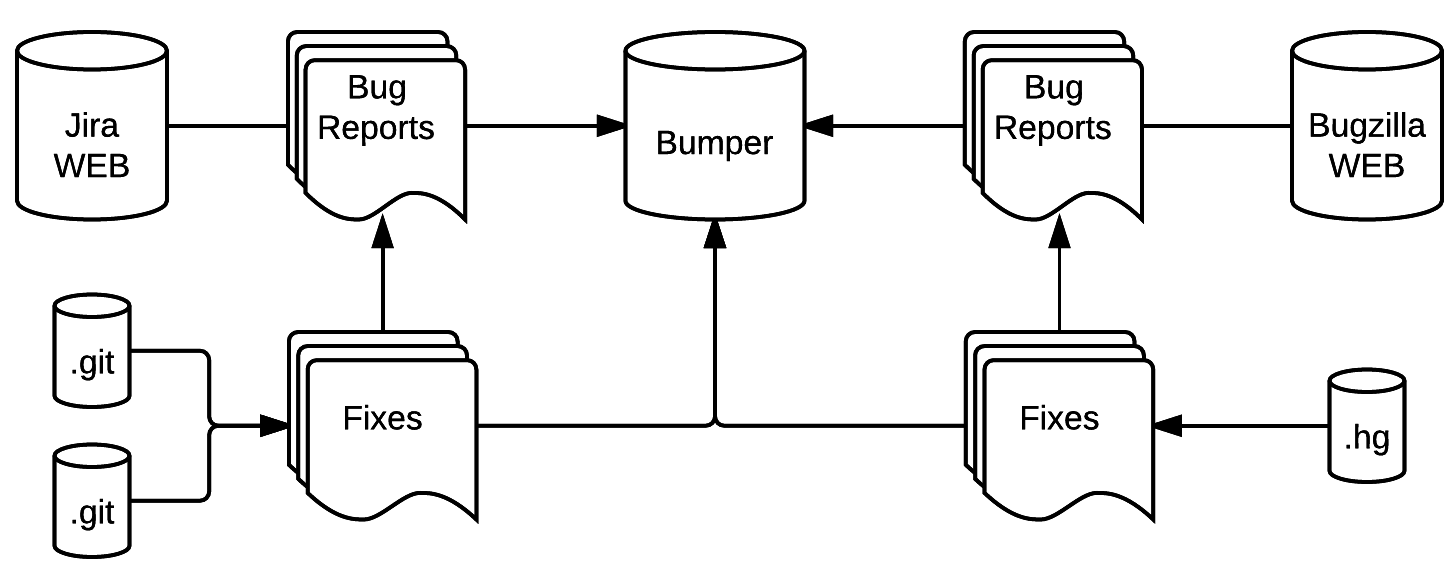
\includegraphics[width=0.4\textwidth]{media/dc.png}
    \caption{Overview of the bumper database construction.\label{fig:data-collection}}
\end{figure}

First, we extract the raw data from bug report management systems of five different open source institutions used in this study: Gnome, Eclipse, Netbeans, Apache Software Foundation and Github.
Each institution is composed of many open source projects: 10, 192, 39, 349 and 250, respectively. Summing up to 840 different open source projects.

The extracted data is consolidated in one database where we associate each bug report with its fix.
The fixes are mined from different types of source versioning system.
Indeed, Gnome, Eclipse and Apache Software Foundation projects are based on Git (or have git based mirrors) while Netbeans uses Mercurial.

Gnome is a free desktop environment mainly developed in c and c++ by volunteers and paid contributors both.

Eclipse and Netbeans are integrated development environments (IDEs) for developing with many programming languages including Java, PHP, and C/C++.

The Apache Software Foundation (ASF) is a non-profit public charity established in 1999, that provides services and support for many like-minded software project communities of individuals who choose to join the ASF.

Finally, Github is a free web-based Git repository hosting service that allow anyone to create, version and maintain a team development project while using Git as source code management and Github issues as Bug management system.

The characteristics of the five dataset used in this paper are presented in Table~\ref{tab:summary}.
Cumulatively, these datasets span from 2001 to 2014.

\begin{table}[]
\centering
\caption{
RESOLVED/FIXED BUG (R/F BR),  CHANGSETS (CS), AND
PROJECTS BY DATASET}
\label{tab:summary}
\begin{tabular}{c|c|c|c|c}
\textbf{Dataset} & \textbf{R/F BR} & \textbf{CS} & \textbf{Files} & \textbf{Projects} \\ \hline \hline
Gnome            &                 &             &                & 10                \\ \hline
Netbeans         & 53,258          & 122,632     & 30,595         & 39                \\ \hline
Apache           & 49,449          & 106,366     & 38,111         & 349               \\ \hline
Eclipse          &                 &             &                & 192               \\ \hline
Github           &                 &             &                & 250               \\ \hline
Total            &                 &             &                & 840               \\ \hline \hline
\end{tabular}
\end{table}

In summary, our consolidated dataset contains 102,707 bugs, 229,153 changesets, 68,809 files that have been modified to fix the bugs, 462,848 comments, and 388 distinct software tools.
We also collected 221 million lines of code impacted by the changesets, identified 3,284 sub-projects, and 17,984 unique contributors to these bug report systems.

We choose these five datasets because they exposed a great diversity in programming languages, teams, localization, utility and maturity.
Moreover, the used different tools, i.e.
Bugzilla, JIRA, Git and Mercurial, and therefore, BUMPER is ready to host any other datasets that used any composition of these tools.

BUMPER users can follow the same process to add other
repositories from various bug tracking and control version
systems such as Eclipse, Mozilla Foundation datasets. The BUMPER architecture can then be used to organize and
access multiple repositories in a unified manner.

\section{Experiments}
\label{sec:Experiments}

In order to assess the efficiency of BUMPER during the debugging / maintenance processes we conduct in which we present participants of the surveys presented in Section \ref{sec:Tools and methods used to fix unknown bug} with a bug to fix.
Then, we ask them to find a suitable solution of the presented bug online as would have in a classical debugging / maintenance session and repeat the operation using BUMPER.
Finally, participants were asked to report how long it took to find a suitable solution with both methods and to rate their experience using BUMPER.

In the remaining of this section we present the three different bugs we randomly submitted to our participant in Section \ref{sub:Bugs to fix}. Then, we describe the time to find a solution reported by our participants and present some of their comments in Sections \ref{sub:Time to find a solution} and \ref{sub:Users comments}, respectively.

\subsection{Bugs to fix}
\label{sub:Bugs to fix}

\subsection{Time to find a solution}
\label{sub:Time to find a solution}

\subsection{Users comments}
\label{sub:Users comments}

\section{Research Oportunities}
\label{sec:Research Oportunities}

In this section we present several research opportunities that BUMPER supports in addition to enhance the debugging / maintenance processes.

\subsection{???}
\label{sub:???}

\subsection{???}
\label{sub:???}

\subsection{Studying bug-fix relationship}
\label{sub:Studying bug-fix relationship}

Studying software repositories to gain insight into the quality of the code is a common practice.
However, this task requires time and skills in order to download and link all the pieces of informations needed for adequate mining.
BUMPER provides a straightforward interface to export bugs and their fixes into CSV, XML and JSON.
As an example, if one wants to extract the features of a bug report that get fixed quickly (this type of analysis is performed in \cite{Bettenburg2008}), the following query can be used:

\begin{equation}
\begin{split}
(type:"BUG"~AND~fixing_time:[0 TO 10]~–churns:0) \\
~OR~(type:"BUG"~AND~fixing\_time:[200~TO~*] \\ –churns:0)\&facet=true\&facet.field=project
\end{split}
\end{equation}

The query returns bugs that have been fixed in less than 10 days and bugs that have been fixed in more than 200 days.
Moreover, the $&facet=true&facet.field=project$ part of the query provides a count of each category (e.g., less than 10 days and more than 200 days) by projects.
Finally, researchers can press the XML, CSV or JSON button, shown in Figure 1. to export their data in the desired format.
In short, BUMPER offers a framework that can be used by software practitioners and researchers to analyze (efficiently) bugs and their fixes without having to go from one repository to another, worry about the way data is represented and saved, or create tools for parsing and retrieving various data attributes.
We hope that the community contributes by adding more repositories to BUMPER. This way, BUMPER can become a unified environment that can facilitate bug analysis and mining tasks.


\section{Related Works}
\label{sec:Related Works}

In last decade, studying the software history in order to improve software maintenance tasks has become popular among researchers and practitioners.
Researchers have specified what makes a good bug report \cite{Bettenburg2008}, studied who should and how long it will take to fix a given bug [12][13].
In addition, researchers have investigated how to resolve the discrepancies between the source code revision system and the bug tracking system \cite{Wu2011} \cite{Antoniol2002} \cite{Bachmann2010} \cite{Bird2010} and how to extract and generate fix patterns \cite{Kim2013} \cite{Pan2008}.
Panoply of approaches and tools built upon this data have also been assessed \cite{Bird2009}, \cite{Bachmann2009a}.
In parallel tools and algorithms to predict or prevent bug insertions that rely on pre-defined bug pattern, theorem proving, model checking or past history have been created \cite{Dangel2000} \cite{Hovemeyer2007} \cite{Kim2007} \cite{Kim2006a}.

However, to the best of our knowledge, no attempt has been made towards building an unified and online datasets, from multiple sources, where all the information related to a bug, or a fix can be easily accessed by researchers and engineers in order to leverage decades of historical information.
Providing a unified, online, and easily accessible datasets has been shown to be effective for learning new APIs \cite{Montandon2013} \cite{Rahman2013} \cite{Kim2011} and BUMPER aims to achieve a similar goal, which is empowering developers by giving access to multiple data repositories that they can use to find how similar bugs have been fixed throughout the history of hundreds of wellknown software projects.


\section{Conclusion}
\label{sec:conclusion}

In this paper, we presented an online tool named BUMPER (BUg Metarepository for dEvelopers and Researchers) accessible at https://bumper-app.com. BUMPER allows natural language searches in bugs reports, commit messages and source code all together while supporting complex queries and contain 380 projects, more than 100,000 resolved/fixed and with 60,000 changesets that were involved in fixing them from Netbeans and The Apache Software foundation’s software.

The speed of BUMPER allows developers to use it as a way to leverage decades of history scattered over hundreds of software project in order to find existing solutions to their problems. As future work, we want to improve BUMPER by adding more projects such as Eclipse, Mozilla Foundation datasets.
Also, we intend to add other features to our bugs report such as the amount of reopening or the number of time a bug has been duplicated.


% use section* for acknowledgment
\section*{Acknowledgment}


The authors would like to thank Ecole de Technologie Superieur Montreal's, Concordia University's, UQAM's and eXia's computer science students and Ubisoft's, Ericsson's, Morgan Stanley's, OVH's, 60fps' and Borealys' developers for participating in our surveys and helping us understanding their day to day needs.


\bibliographystyle{IEEEtran}
\bibliography{library.bib}


\end{document}
